\section{Trust-Related Behaviors}
add stuff
\subsection{Calibration of Trust-Related Behaviors}
    As yet, trust is not a quantity that can be directly measured. Rather, its relative magnitude must be observed through changes in TRBs. \citet{Parasuraman1997-co} were interested in understanding the use of automation which they defined as ``\ldots the execution by a machine agent (usually a computer) of a function that was previously carried out by a human''. Within this scope they define the following terms: a) \emph{misuse}, the overreliance on automation, b) \emph{disuse}, the underutilization of automation, and c) \emph{abuse}, inappropriate application of automation.

    Here it is proposed that, analogously, the definitions of \emph{misuse}, \emph{disuse}, and \emph{abuse} can apply to the relationship between humans and autonomy (where autonomy is defined as a system, such as an artificial agent with processing power possibly located on a physical robot, that is able to independently act in uncertain environments to accomplish a goal).
    
    To be more formal, let the total set of TRBs as $\mathcal{T}$. Then as subsets of $\mathcal{T}$ define the set of misue actions as $\mathcal{M}$, the set of disuse actions as $\mathcal{D}$, and the set of abuse actions as $\mathcal{A}$. Next, define the total set of innapropriate TRBs $\mathcal{I}$ as the union of $\mathcal{I} = \mathcal{M}\cup \mathcal{D}\cup\mathcal{A}$. Having defined the set of inappropriate actions, the set of appropriate TRBs can be defined as $\mathcal{U}$, the compliment of the set of inappropriate TRBs $\mathcal{U} = \mathcal{I}^\prime$. This is illustrated in Figure \ref{fig:appropriate_use}, where the set of appropriate actions $\mathcal{U}$ is the gray colored area (i.e. all TRBs \emph{not} in either of the three sets of inappropriate TRBs).
    
	\begin{figure}[htbp]
    	\centering
     	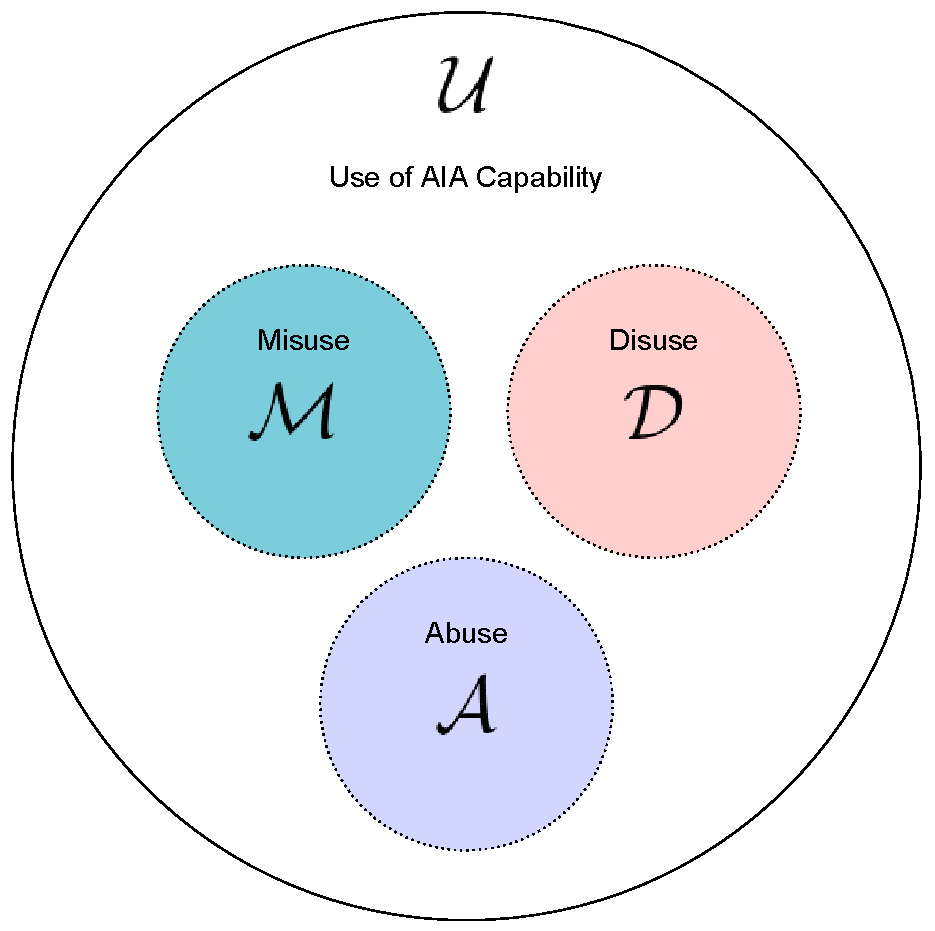
\includegraphics[width=0.4\textwidth]{Figures/misuse_disuse_abuse}
    	\caption{Graphic representing the total space of user actions, in which the inappropriate uses $\mathcal{M}$, $\mathcal{D}$, and $\mathcal{A}$ lie. The set of inappropriate uses $\mathcal{I}$ is the union of $\mathcal{M}$, $\mathcal{D}$, and $\mathcal{A}$. The appropriate set of actions $\mathcal{U}$ is the compliment of \mathcal{I}, or the part of $\mathcal{T}$ that does not include $\mathcal{I}$.}
        \label{fig:appropriate_use}
    \end{figure}
    
    In order to ensure that humans use autonomous systems appropriately it is critical that the user TRBs be calibrated to elicit behaviors that are within $\mathcal{U}$. This can be done by influencing the user trust.

    Generally trust between a human and AI could be depicted as in Figure \ref{fig:SimpleTrust_two_way}, where each has TRBs that must be calibrated, and each provides certain feedback, which will be called assurances, in order to do so. In a more simple scenario, where the AI implicitly trusts the human user the trust relationship can be depicted as shown in Figure \ref{fig:SimpleTrust_one_way}, where only the user has TRBs that are being calibrated.

	\begin{figure*}[htbp]
        \centering
        \begin{subfigure}[t]{0.48\textwidth}
            \centering
            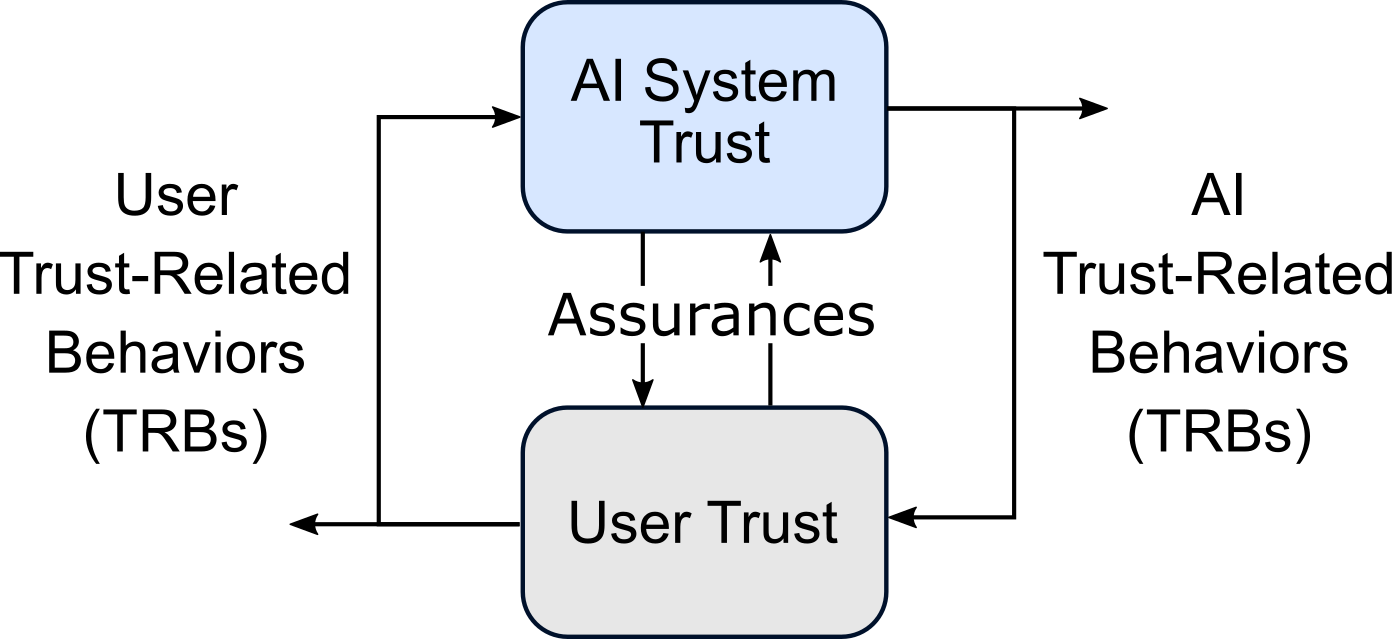
\includegraphics[width=0.95\textwidth]{Figures/SimpleTrust_two_way}
            \caption{Diagram showing a general case of a two-way trust relationship between an AI and a human. Arrows that are not connected to boxes represent some action outside of the trust loop.} 
            \label{fig:SimpleTrust_two_way}%
        \end{subfigure}
        \hfill
        \begin{subfigure}[t]{0.48\textwidth}
            \centering
            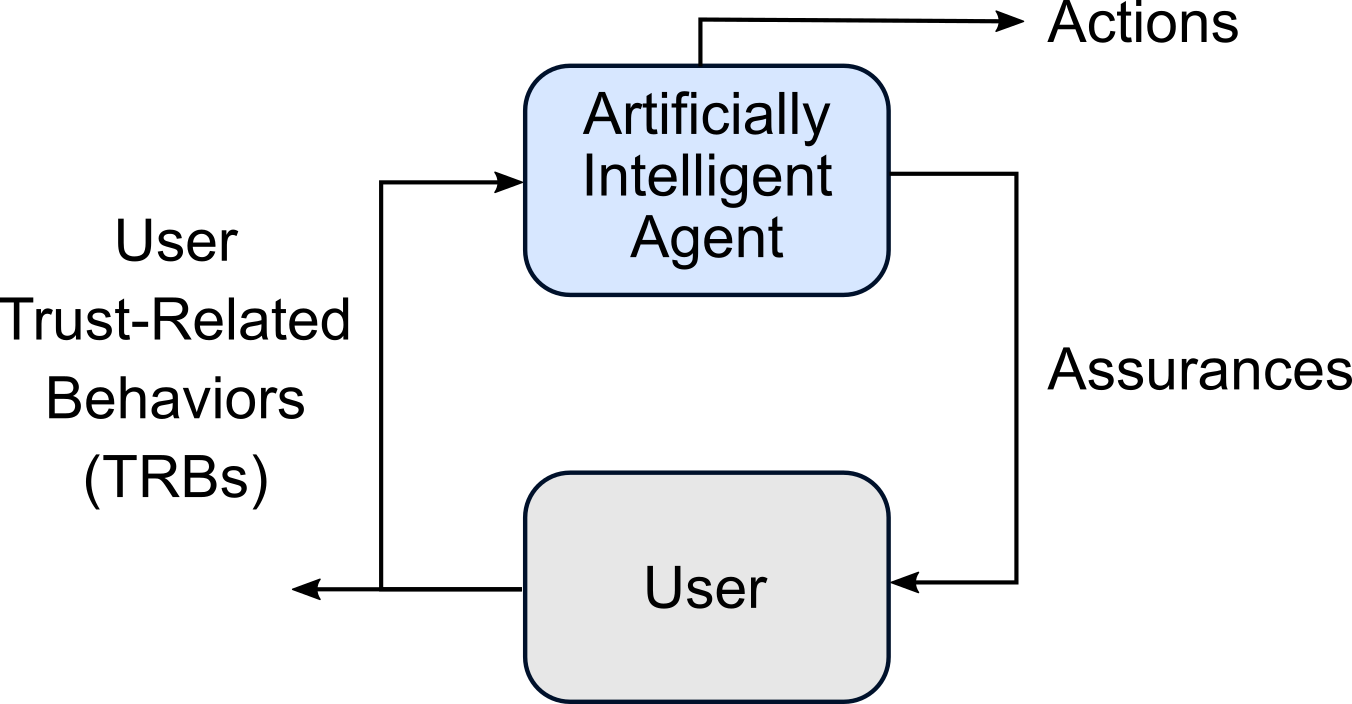
\includegraphics[width=0.95\textwidth]{Figures/SimpleTrust_one_way}
            \caption{Diagram illustrating a general one-way trust relationship between a human and an AI. In this case the AI has, what could be considered perfect trust in the user.}
            \label{fig:SimpleTrust_one_way}%
        \end{subfigure}
        \caption{Feedback Loops For One and Two-way human-AI Trust Relationships}
        \label{fig:SimpleTrust}
    \end{figure}
    
    Figure \ref{fig:SimpleTrust_dist} serves as a simple example illustrating the possible disparity between the user TRB distribution and the appropriate TRB distribution. In this case assurances would be used to minimize the difference between the two distributions.

	\begin{figure}[htbp]
    	\centering
     	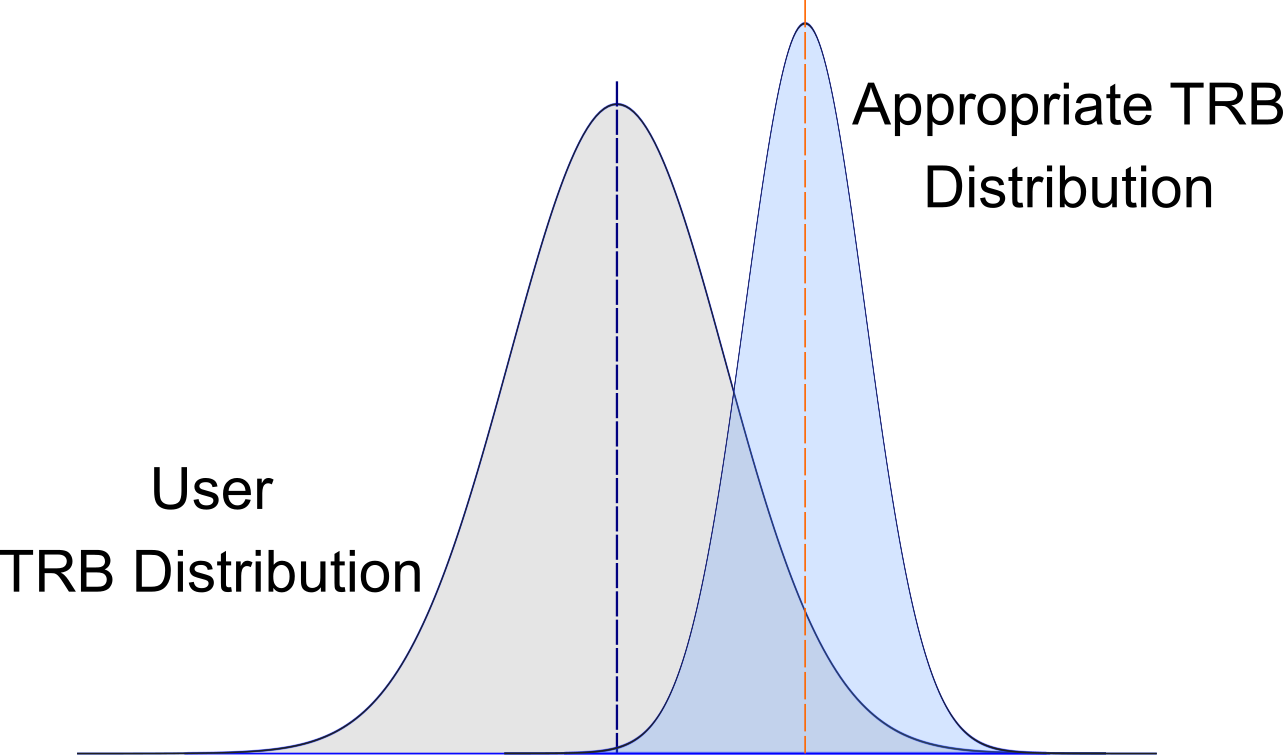
\includegraphics[width=0.4\textwidth]{Figures/SimpleTrust_dist.png}
    	\caption{Diagram illustrating the point that a hypothetical user TRB distribution might not match the appropriate TRB distribution. In this case the AI should provide assurances in order to minimize the difference between the two.}
        \label{fig:SimpleTrust_dist}
    \end{figure}

